\documentclass{article}

\usepackage{amsmath, amsfonts}
\usepackage{graphicx}
%\usepackage{subcaption}
\usepackage{csvsimple}
\usepackage{comment}

\usepackage[parfill]{parskip}

\begin{document}

\title{Report Outline}
\author{Fabian}

\maketitle

\section{Introduction}
A short introduction to the field of load forecasting and its relevance.\\
Description of the competition.

\section{Review of related Work}
Review previous work from Gefcom 2012 including papers with related approaches including but not limited to those that can be found under the following link: http://blog.drhongtao.com/2014/08/recommended-papers-for-gefcom2014-contestants.html. Distinguish between approaches to temperature and load prediction.\par

Probabilistic Electric Load Forecasting: A Tutorial Review
https://onedrive.live.com/view.aspx?resid=BCA4C2DC57A4CB2A!519&app=WordPdf
contains literature review for longterm probabilistic load forecasting

Tao Hang, Jason Wilson:
Long Term Probabilistic Load Forecasting and Normalization With Hourly Information
but papers is on Long Term Electric Load Forecasting: 1-X years

\section{Data}
Description of the data made available for the competition
\subsection{Temperature Data}
\begin{comment}
\begin{table}[h!]
\centering
\begin{tabular}{llllll}
Year & Mean        & Median & StD         & Min   & Max   \\
2001 & 60.72339045 & 62.2   & 15.16199974 & 16.96 & 93.44 \\
2002 & 61.61707306 & 63.64  & 16.25871076 & 21.6  & 95.76 \\
2003 & 59.86723744 & 61.92  & 15.72253502 & 13.96 & 91.56 \\
2004 & 60.60986794 & 63.6   & 16.20390846 & 14.6  & 91.6  \\
2005 & 60.72554795 & 62.62  & 16.47735821 & 15.12 & 97.4  \\
2006 & 61.17943836 & 62.22  & 14.84796583 & 20.48 & 94.96 \\
2007 & 61.76222831 & 63.76  & 16.05569468 & 17.96 & 97.68 \\
2008 & 60.73573315 & 61.84  & 15.58815285 & 17.92 & 96.12 \\
2009 & 60.33642466 & 62.28  & 15.88100762 & 12.64 & 93.12 \\
2010 & 60.16820091 & 63.16  & 18.50289712 & 16.6  & 97.44 \\
2011 & 62.6862927  & 65.32  & 16.28001634 & 17.84 & 96.48
\end{tabular}
\caption{Yearly basic statistics for average temperature over 25 weather stations in Fahrenheit}
\end{table}
\end{comment}
The temperature data made available consists of 25 series of temperature data in Fahrenheit from 25 different weather statios dating from 01/01/2001 to 12/01/2011.\\
%$Corr_X(m) = \frac{\mathbb{E}\[X_t-\mu_x)(X_{t+m})\]}{\var_X}$
The Cross Correlation of the different temperature series with each other suggest that they can be explained to over 90\% by the first series. [include correlation plots]
If we assume a temperature of 60 degrees fahrenheit, that would allow for an error of maximum 6 degrees of fahrenheit or 3 degrees celsius. As we will see later this error is negligable given the inaccuracy of the temperature prediction.

\subsection{Load Data}
\begin{comment}
Some basic statistics computed by year.
\begin{table}[!h]
\centering
\begin{tabular}{llllll}
Year & Mean        & Median & StD         & Min  & Max   \\
2005 & 139.1157985 & 129.4  & 44.46885208 & 64.8 & 291.3 \\
2006 & 134.5321005 & 125    & 42.01147924 & 48.4 & 291.4 \\
2007 & 144.4574772 & 134.8  & 44.64622456 & 69   & 307.4 \\
2008 & 147.095526  & 134.9  & 45.84668098 & 72.5 & 295.9 \\
2009 & 149.1644292 & 139.2  & 44.95448884 & 64.4 & 303.8 \\
2010 & 161.1352055 & 150.3  & 52.87939039 & 72.4 & 315.6 \\
2011 & 148.4394041 & 135.25 & 50.07312759 & 16.1 & 317.5
\end{tabular}
\caption{Yearly basic statistics for Energy Load in Mega Watts}
\end{table}
\end{comment}

\subsubsection{"Lag Analysis"}
The effect of the lag on the Time Series Correlation Coefficient can be demonstrated using the Autocorrelation function acf() built into R stats. Here we display five plots showing the Autocorrelation Function for different maximum lags: 
\begin{figure}[h!]
\centering
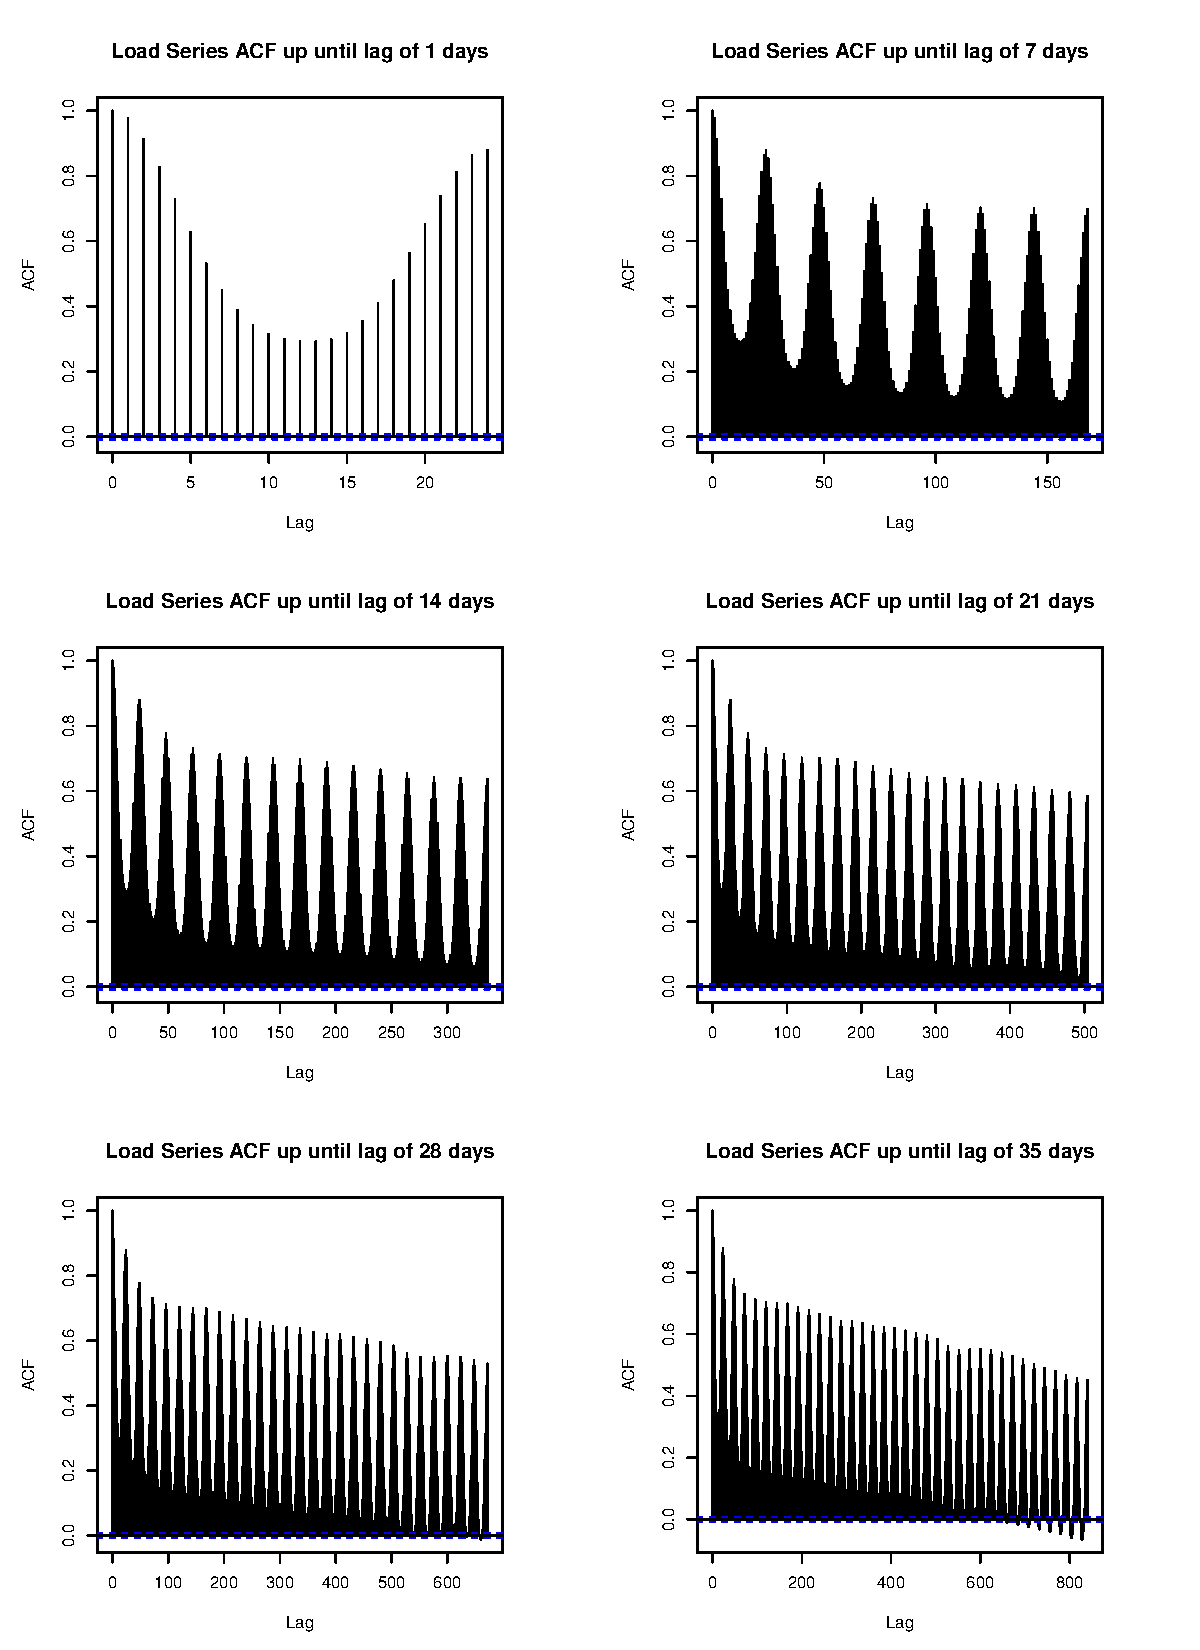
\includegraphics[width=.7\textwidth]{../data/analysis/acf-load-lag-var-days_font.pdf}
\caption{Plots of Autocorrelation Function estimates of hourly load data in Mega Watts for different maximum lags.}
\label{fig:load-acf}
\end{figure}

As can be seen the correlation diminishes exponentially up until a lag of 72h from any point in the time series, then stays more or less constant for up to 7-8 days, whereafter it diminishes near linearly (up to a lag of 35 days). 
\subsection{Basic exploration with Time Series Analysis Methods}
Autocorrelation, include decompositions? (included in "Data")

\section{Feature 'Extraction'}
Description of the features obtained from the data. 
\subsection{Calendar Features}
hour, TOY vs. month

\section{Models}
Description of the Models (LM), GAM (more extensive), NN, RF

\section{Analysis}
What combination of features and models for temperature and load provide us with a good prediction accuracy with respect to Gefcom leaderboard?

\subsection{Error Measures}
Introduce error measures (RMSE, MAE, MAPE, PINBALL) and their differences here? Too late?

\subsection{Temperature Modeling}
\subsubsection{Data Processing}
average temperature vs. principal component

\subsubsection{Effect on Load Prediction}
Effect of temperature on load prediction evaluated using different methods:\\
Mean over past years (yearly lag), LM, GAM, NN, RF vs. true temperature

\subsubsection{Evaluate Results of weekly vs. monthly Temperature Prediction}
plot MAPE \& PINBALL scores for different methods over load training + CV period in a 1x2 plot of the form:\\
monthly scores \quad weekly scores

\subsection{Load Modeling}

\subsubsection{Evaluate the Influence of the Lag on Load Prediction}
set the basis by plotting MAPE \& PINBALL scores by week over w1, w2, w3, w4; one curve for every month in CV\\
do this for every method\\
as well as a comparison of the best performing configuration of every method among each other\\

\subsubsection{Evaluate Performance for different Method Configurations}
Use temp method that provides best score as shown in Temperature Modeling Section\par
Different GAM formulas:\\
plot MAPE \& PINBALL scores for all GAM formulas over CV period in a 2x2 plot of the form:\\
monthly load with monthly temp \quad monthly load with weekly temp\\
weekly load with monhtly temp \quad weekly load with weekly temp\par
\vspace*{5pt}
Different NN hidden units:\\
plot MAPE \& PINBALL scores in 2x2 plot\par
Different RF ntrees:\\ 
plot MAPE \& PINBALL scores in 2x2 plot\par

\subsubsection{Compare Performance of different Methods}
choose best scoring configuration for every method and plot the results in one 2x2 plot

\section{Conclusion}
Draw conclusion based on the analysis done in the main part.

\end{document}